%%%%%%%%%%%%%%%%%%%%%%%%%%%%%%%%%%%%%%%%%%%%%%%%%%%%%
\chapter{Combination of searches for diboson resonances at $\sqrt{s}$ = 8 and 13 TeV}
\label{ch:combination}
%%%%%%%%%%%%%%%%%%%%%%%%%%%%%%%%%%%%%%%%%%%%%%%%%%%%%

In addition to the analyses described in this work, several similar searches for heavy resonances decaying to pairs of W, Z, and Higgs bosons in various final states have been performed with the CMS experiments in both LHC Run 1 and Run 2~\cite{CMS-PAS-EXO-15-002,Khachatryan:2016cfx,Khachatryan:2014gha, Khachatryan:2014hpa, Khachatryan:2015bma, Khachatryan:2014xja,Khachatryan:2016yji,Khachatryan:2015ywa}.
As these searches have individually very similar sensitivity to benchmark physics scenarios of interest, a statistical combination to maximize the overall sensitivity is performed and presented in this Chapter.
Furthermore, the combination of these analyses is fundamental to fully understand the compatibility of the excess observed in the $\ell\Pgn\bbbar$ final state at \mWH = 1.8\TeV as discussed in Chapter~\ref{ch:results8}.
The interest in this excess has been further enhanced by the observation of an excess at the same diboson invariant mass values by ATLAS in the all-hadronic VV final state~\cite{Aad:2015owa}.

The analyses taken into account in the statistical combination are based on pp collision data collected by the CMS experiment during 2012 and 2015 at $\sqrt{s} = \unit{8}{\TeV}$ and $\unit{13}{\TeV}$, corresponding to an integrated luminosity of \unit{19.7}{\fbinv} and \unit{2.3}--\unit{2.7}{\fbinv}, respectively.
Analyses with all-leptonic, semi-leptonic, and all-jets final states are considered. This includes the decay into charged leptons ($\ell$) and neutrinos ($\Pgn$) of W and Z bosons, as well as reconstructed jets containing the decay products of hadronically decaying W or Z bosons. The latter are labeled as \qqbar final states that include $\rm W\to\qqbar'\to$~jet and $\rm Z\to\qqbar\to$~jet. For Higgs bosons, hadronic decays labeled as \bbbar or $\qqbar\qqbar$ final states referring to $\rm H\to\bbbar$ or $\rm H\to\qqbar'\qqbar'$ are considered.

Altogether, results are combined corresponding to the following final states: $\ell \Pgn \qqbar$ (13 TeV)~\cite{CMS-PAS-EXO-15-002}, $\qqbar \qqbar$ (13 TeV)~\cite{CMS-PAS-EXO-15-002},
$\ell \ell \bbbar$/$\ell \Pgn \bbbar$/$\Pgn \Pgn \bbbar$ (13 TeV)~\cite{Khachatryan:2016cfx},
3$\ell\Pgn$ (8 TeV)~\cite{Khachatryan:2014xja}, 
$\ell \Pgn \qqbar$ (8 TeV)~\cite{Khachatryan:2014gha}, $\ell\ell \qqbar$ (8 TeV)~\cite{Khachatryan:2014gha}, 
$\qqbar \qqbar$ (8 TeV)~\cite{Khachatryan:2014hpa}, 
$\ell \Pgn \bbbar$ (8 TeV)~\cite{Khachatryan:2016yji}, $\qqbar\bbbar/6$q (8 TeV)~\cite{Khachatryan:2015bma}, 
$\qqbar \tau\tau $ (8 TeV)~\cite{Khachatryan:2015ywa}.

The results are interpreted in the context of the BSM models described in Section~\ref{sec:BSMintro}, namely, heavy vector triplet and singlet models predicting $\Wpr$ and $\Zpr$ bosons, and the bulk graviton model.
Combined cross section limits as a function of resonance mass are obtained. This is the first combined search for high mass resonances with both WW/WZ and WH/ZH signatures.
%As the experimental signature of hadronically decaying W and Z bosons cannot fully be discriminated given the experimental jet mass resolution,
%analyses can be sensitive to multiple signals predicted by the same model. The final state $\ell \Pgn \qqbar$ is for example sensitive to a HVT $\Wpr$ decay to WZ as well as to $\Zpr$ decaying to WW.
%This contribution of multiple signals to the same analysis is therefore taken into account in the combination.
%For this reason separate interpretations for a vector triplet ($\Wpr$ and $\Zpr$) and for vector singlets ($\Wpr$ or $\Zpr$) are presented.

A summary of the analyses entering the combination is given in Section~\ref{sec:analyses}.
The combination procedure is described in Section~\ref{sec:combination}, and finally the results are presented and discussed in Section~\ref{sec:comboResults}.

%%%%%%%%%%%%%%%%%%%%%%%%%%%%%%%%%%
\section{Inputs to the combination}\label{sec:analyses}
%%%%%%%%%%%%%%%%%%%%%%%%%%%%%%%%%%

A statistical combination is carried out of searches for new heavy resonances that are performed on top of the steeply falling invariant mass distribution of two reconstructed W, Z or Higgs bosons. Various decay modes of these bosons are considered.
The $\rm Z\to \ell\ell$ candidates are reconstructed from electron and muon candidates, while $\rm W \to \ell$$\Pgn$ candidates are reconstructed from identified muons or electrons with the method described in Section~\ref{sec:leptonicW}, which makes use 
of the missing transverse momentum under the constraint that the $\ell$$\Pgn$ invariant mass is equal to the known W-boson mass.
The $\rm H\to$$\tau\tau$ candidates are reconstructed from electron, muon and hadronically-decaying tau candidates in combination with missing transverse momentum.
The $\rm W\to \qqbar'$, $\rm Z\to \qqbar$, $\rm H\to \bbbar$ and $\rm H\to \qqbar'\qqbar'$ candidates are reconstructed with jet algorithms with a distance parameter of 0.8 (CA for the 8 TeV data analyses, AK for the 13 TeV analyses). 

All analyses are focused on high mass resonances which decay in highly boosted W/Z/H bosons. Hence, their decay products are reconstructed close-by in angle, requiring special reconstruction techniques.
For highly boosted W/Z/H bosons decaying to electron, muon and tau candidates, identification and isolation requirements are adapted such that the nearby reconstructed leptons do not reduce the identification efficiency.

For highly boosted V bosons decaying to quark anti-quark pairs, the V algorithm described in Section~\ref{sec:vtagging} is applied.
In the 8 TeV data analyses, a V jet candidate is identified if its pruned mass, \mJ, falls in a range around the W or Z mass.
In the 13 TeV data analyses, two distinct categories enriched in W or Z bosons are defined by two exclusive ranges in \mJ as described in Section~\ref{sec:finalselection}.
In the 8\TeV data analyses the sensitivity is further enhanced by distinguishing two categories, a low purity (LP) and a high purity (HP) one based on the $\tau_{21}$ variable.
This same strategy is follow in the dijet 13\TeV analysis. Although the HP category dominates the total sensitivity of the analyses, the LP category is retained,
since for large masses of a new resonance it provides improved signal efficiency with only moderate background contamination.

Higgs-boson identification is similarly performed using a pruned jet mass window around the Higgs mass together with b-tagging algorithms applied to the H jet or to its subjets as described in Section~\ref{sec:htagging}.
To distinguish $\rm H\to \rm W\rm W\to \qqbar'\qqbar'$ jets from background, a similar technique as V tagging is applied using the $\tau_{42}$ ratio. The selection efficiencies for each signal and channel are summarized in Table~\ref{tab:efficiencies}.

\begin{table}[!htb]
  \centering
  \caption{Summary of the signal efficiencies of all analysis channels for all signal models for a 2 TeV resonance.
For analyses with categorization in high-purity (HP) and low-purity (LP) categories, both efficiencies are quoted in the form HP/LP.
The signal efficiencies are in percent and include the SM branching ratios of the bosons to the final state of the analysis channel,
effects from detector acceptance, as well as reconstruction and selection efficiencies.
%Numbers in brackets indicate small signal contributions that are not considered in the overall combination.
}
  \begin{tabular}{l|c c|c c|c c}
    \hline
 Channel & \multicolumn{4}{c|}{HVT} & \multicolumn{2}{c}{RS bulk} \\
  & \multicolumn{2}{c|}{$W'$} & \multicolumn{2}{c|}{$Z'$} & \multicolumn{2}{c}{$\rm G_{bulk}$} \\
  & WZ & WH & WW & ZH & WW & ZZ \\
    \hline
 3$\ell\Pgn$ (8 TeV) & 0.6 & - & - & - & - & -\\   
 $\ell\ell \qqbar$ (8 TeV) &  1.1/- &  - &  - &  0.2/- &  - &  3.0/1.0\\
 $\ell \Pgn \qqbar$ (8 TeV) &  4.8/- &  - &  9.4/- &  - &  10.6/7.1 &  -\\
 $\qqbar \qqbar$ (8 TeV) &  5.9/5.5 &  0.8/0.7 &  5.7/5.3 & 0.8/0.7 &  3.8/3.1 &  5.7/4.2\\
    \hline
 $\ell \Pgn \bbbar$(8 TeV) &  - &  0.9 &  - &  - &  - &  -\\
 $\qqbar \tau\tau$ (8 TeV)  &  - &  1.2 &  - &  1.3 &  - &  -\\
 $\qqbar\bbbar/6$q (8 TeV) &  - &  3.0/1.8 &  - &  1.7/1.1 &  - &  -\\
    \hline
 $\ell \Pgn \qqbar$ (13 TeV) &  10.2/- &  1.7/- &  19.4/- &  - &  18.1/- &  -\\
 $\qqbar \qqbar$ (13 TeV) &  9.7/12.3 &  1.8/2.5 &  8.2/10.6 & 1.9/2.6 &  8.7/12.4 &  11.0/13.5\\
    \hline
 $\ell\ell\bbbar$ (13 TeV) &  - &  - &  - &  1.5 &  - &  -\\
 $\ell\Pgn\bbbar$ (13 TeV) &  - &  4.0 &  - &  - &  - &  -\\
 $\Pgn\Pgn\bbbar$ (13 TeV)  &  - &  - &  - &  4.2 &  - &  -\\
   \hline
  \end{tabular}
  \label{tab:efficiencies}
\end{table}

In all-jets final states, the background dominated by QCD multijets production is estimated with a fit of signal+background to the data, where the background is described by a smooth functional form.
In semi-leptonic final states, the dominant backgrounds from V+jets production are estimated using data in $\mJ$ sidebands with the method described in Section~\ref{sec:alpha}.
In all-leptonic final states, the dominant background from standard model diboson production is estimated using simulated events.

More details are given in the following for the analyses where not all signal models presented in the combination were originally originally considered.

%%%%%
\subsection{Reinterpretations}
%%%%%

In the searches for new heavy resonances decaying into a pair of vector bosons (WW, ZZ or WZ) in the semi-leptonic ($\ell \Pgn \qqbar$ and $\ell\ell \qqbar$) final states~\cite{Khachatryan:2014gha} with pp collision data collected at $\sqrt{s}$ = 8 TeV, exclusion limits at 95\% CL have been set on the production cross section of a bulk graviton.
The results were published with a parametrization for the reconstruction efficiency as a function of W and Z boson kinematics, enabling a reinterpretation in the context of the HVT model B described in Section~\ref{subsec:hvt}, which predicts the production of charged and neutral spin-1 resonances decaying preferably to WW and WZ.
The reinterpretation in the context of this model is obtained by rescaling the bulk graviton signal efficiencies by scale factors taking into account the different kinematics of W and the Z bosons from \PWpr{} and \cPZpr{} production compared to the graviton production.
The scale factors have been derived for each mass point by means of the tables published in Ref.~\cite{Khachatryan:2014gha}.
Since the efficiency parametrization is restricted to the HP category of the analyses, the LP category is not used for the HVT \PWpr{} and \cPZpr{} interpretations of these channels.
The \mJ window that defines the signal regions of the analysis channels is such that the $\ell \Pgn \qqbar$ channel is sensitive to both the charged and neutral resonance predicted by HVT models. This is taken into account in the combination presented in Section~\ref{subsec:comboHVT}.

The searches for new heavy resonances decaying into a pair of vector bosons (WW, ZZ or WZ) in the semi-leptonic ($\ell \Pgn \qqbar$ and $\ell\ell \qqbar$)~\cite{Khachatryan:2014gha,Khachatryan:2014gha,CMS-PAS-EXO-15-002}, and all-hadronic ($\qqbar \qqbar$) final states~\cite{Khachatryan:2014hpa,CMS-PAS-EXO-15-002} at 8 and 13 TeV, are also sensitive to WH and ZH signatures, since a small fraction of jets initiated by Higgs bosons have a pruned jet mass in the range considered to identify W or Z bosons.
These searches were therefore re-interpreted with WH and ZH signals to profit from this additional signal sensitivity.
The additional signal efficiencies for those signals are indicated in Table~\ref{tab:efficiencies}.

The search for resonances in the $\qqbar \tau\tau$ final state~\cite{Khachatryan:2015bma} was optimized for a resonance \Zpr decaying into Z and a Higgs boson.
However, given the large \mJ window ($65~\GeV <  \mJ < 105~\GeV$) used to tag the hadronically decaying Z boson, this analysis channel is also sensitive to the production of the charged spin-1 \Wpr resonance decaying into W and Higgs bosons as predicted in HVT models. This overlap is taken into account in the statistical combination described in Section~\ref{subsec:comboHVT}.

%%%%%%%%%%%%%%%%%%%%%%%%%%%%%%%%%%
\section{Combination procedure}\label{sec:combination}
%%%%%%%%%%%%%%%%%%%%%%%%%%%%%%%%%%

In all the analysis channels a search is performed for a peak on top of the falling background distribution in the diboson invariant mass by means of a maximum likelihood fit to the data.
As done for the main analyses described in this work (Section~\ref{sec:stat}), the likelihood function is maximized to obtain the best fit of the signal strength modified $\mu$ for each signal and resonance mass hypothesis.
The function is constructed from the reconstructed diboson invariant mass distribution observed in data, the background prediction, and the signal resonance shape to test for the presence of a new resonance decaying to two bosons.
For the 3$\ell\Pgn$, $\qqbar \qqbar$, $\qqbar\bbbar/6$q, and $\qqbar \tau\tau $ analyses, the likelihood function is computed using events binned as a function of reconstructed diboson invariant mass as in Equation~\ref{eqn:binned}.
For the remaining analyses ($\ell \Pgn \qqbar$,  $\ell\ell \qqbar$, $\ell \Pgn \bbbar$), the functional form for an unbinned likelihood is similarly defined using functional forms that describe the shape of the reconstructed diboson invariant mass for background and signal resonance as given by Equation~\ref{eqn:unbinned}.

The treatment of the background in the maximum likelihood fit depends on the analysis channel.
In the $\qqbar \qqbar$ and $\qqbar\bbbar/6$q analyses, the background fit function parameters are left floating in the maximum likelihood fit, such that the background prediction is simultaneously obtained with the signal $\mu$ for every hypothesis.
The remaining analyses ($\ell \Pgn \qqbar$,  $\ell\ell \qqbar$, $\ell \ell \bbbar$, $\ell \Pgn \bbbar$, $\Pgn \Pgn \bbbar$) follow the same procedure as for the analyses described in this work: the background is estimated using data sidebands and uncertainties related to its parametrized shape are treated as nuisance parameters constrained with Gaussian probability density functions in the maximum likelihood fit. Except for the cases described in Section~\ref{sec:analyses}, which have been found to be negligible, selection are exclusive. The combined likelihood is then obtained from the product of the likelihoods of each individual analysis channel.

The asymptotic approximation of the $\mathrm{CL_s}$ criterion (Section~\ref{subsec:AsymptCLs}) is used with the test statistic given by Equation~\ref{eqn:testStatistic} to set upper limits on the cross section for resonance production.
When combining 8 and 13\TeV analyses, limits are set on the signal scale factor $\mu$ taking into account the production cross section ratio evaluated from theory between 8\TeV and 13\TeV.

The dominant sources of systematic uncertainties are treated as nuisance parameters constrained with a log-normal probability density function.
All nuisance parameters are profiled following the frequentist convention discussed in Section~\ref{sec:stat}.
When the likelihoods of multiple analyses channels are combined, the correlation of systematic effects across analysis channels is taken into account by categorizing the uncertainties into fully correlated (associate to same nuisance parameter) and fully uncorrelated (associate to different nuisance parameters).
Table~\ref{tab:correlations} summarizes which uncertainties are treated as correlated among 8 and 13\TeV analyses, electron and muon channels, HP and LP categories and W, Z and Higgs enriched categories in the combination.
Further categorisation within individual analyses are described therein.

\begin{table}[htb]
  \centering
  \caption{Correlation of systematic uncertainties.
}
  \begin{tabular}{l l c c c c}
    \hline
    Systematic uncertainty & Type & 8+13 TeV & e+$\mu$ & HP+LP & W+Z+Higgs \\
    \hline
    Lepton trigger & yield & no & no & yes & yes \\
    Lepton identification & yield & no & no & yes & yes \\
    Lepton momentum scale & yield, shape & no & no & yes & yes \\
    Jet energy scale & yield, shape & no & yes & yes & yes \\
    Jet energy resolution & yield, shape & no & yes & yes & yes \\
    Jet mass scale & yield & no & yes & yes & yes \\
    Jet mass resolution & yield & no & yes & yes & yes \\
    b tagging & yield & no & yes & yes & yes \\ 
    W tagging \nsubj{} (HP/LP) & yield & no & yes & yes & yes \\
    Integrated luminosity & yield & no & yes & yes & yes \\
    Pileup & yield & no & yes & yes & yes \\
    PDF & yield & yes & yes & yes & yes \\
    $\mu_{f}$,$\mu_{r}$ scales & yield & yes & yes & yes & yes \\
    \hline
  \end{tabular}
  \label{tab:correlations}
\end{table}

The most important and only nuisance parameters treated as correlated between 8 and 13\TeV analyses are those related to the PDFs and the choice of factorization ($\mu_{f}$) and renormalization ($\mu_{r}$) scales used to estimate the signal cross sections.
They have been re-evaluated for this combination for both 8 and 13\TeV analyses, estimating the full impact on the expected signal yield rather than the impact on only the signal acceptance.
The PDF uncertainties are evaluated using the NNPDF 3.0~\cite{Ball:2011mu} PDFs.
The uncertainty related to the choice of $\mu_{f}$ and $\mu_{r}$ scales is evaluated following the proposal in Refs.~\cite{Cacciari:2003fi,Catani:2003zt} by varying the default choice of scales in the following 6 combinations of factors:
$(\mu_{f}$, $\mu_{r})$ $\times$ $(1/2, 1/2)$, $(1/2, 1)$, $(1,1/2)$, $(2, 2)$, $(2, 1)$, and $(1, 2)$.
The experimental uncertainties are all treated as uncorrelated between 8 and 13\TeV. At 13\TeV the systematic uncertainties are dominated by the statistical uncertainty of the datasets used to evaluate scale factors applied to the signal simulation to reproduce data.

%%%%%%%%%%%%%%%%%%%%%%%%%%%%%%%%%%
\section{Results}\label{sec:comboResults}
%%%%%%%%%%%%%%%%%%%%%%%%%%%%%%%%%%

In this section the combination of the individual analysis channels described in Section~\ref{sec:analyses} is presented, for each of the signal hypothesis described in Section~\ref{sec:BSMintro}.
%summarized in Table~\ref{tab:models}.
For each channel the 95\% CL exclusion limits on the signal strength modifier $\mu = \sigma_{95\%}/\sigma_{\rm theory}$ are presented.

%%%%%
\subsection{Limits on \Wpr and \Zpr singlets}
%%%%%

\begin{figure}[!htb]
\centering
\subfigure[]{\label{fig:wpall_138TeV_a}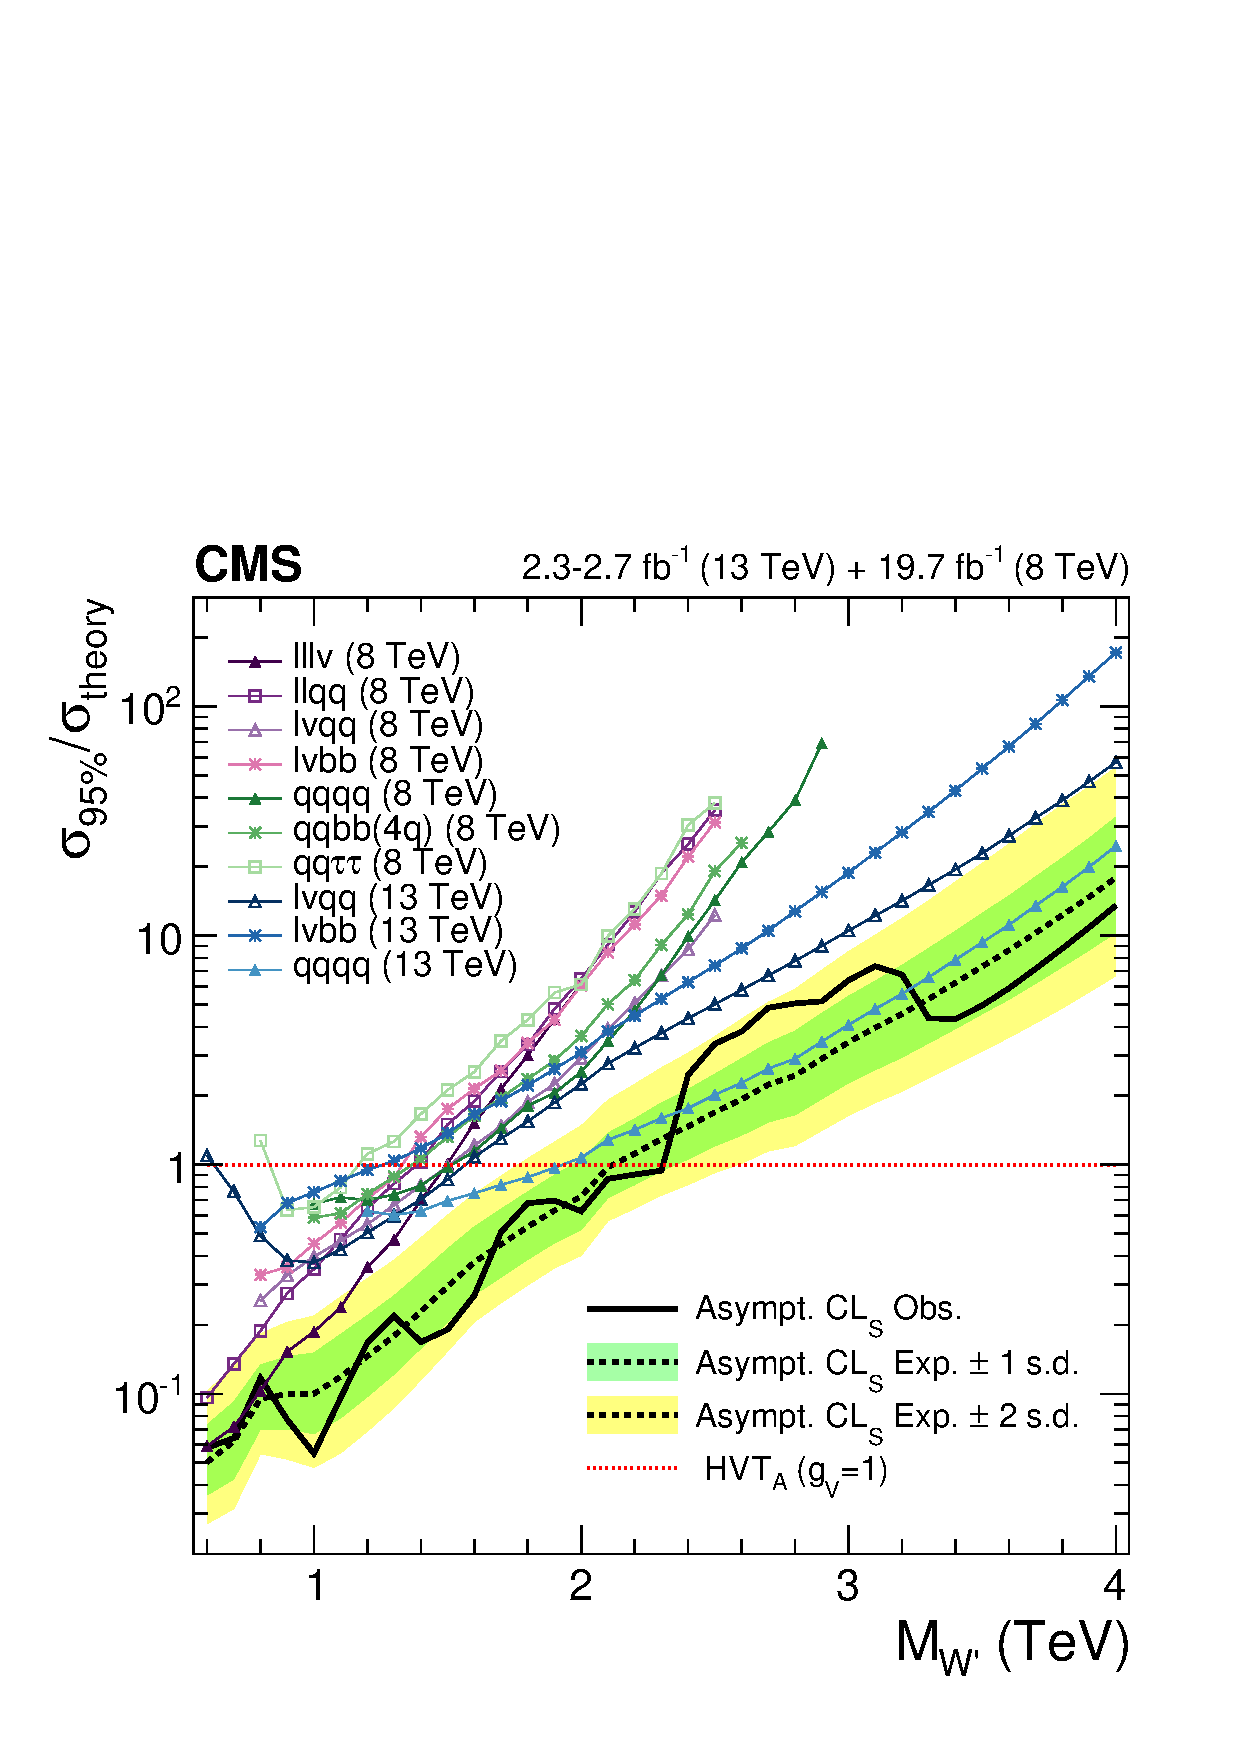
\includegraphics[width=0.45\textwidth]{\cheleven/EXOVVhvta_compare_ALLWPRIME138_final.pdf}}
\subfigure[]{\label{fig:wpall_138TeV_b}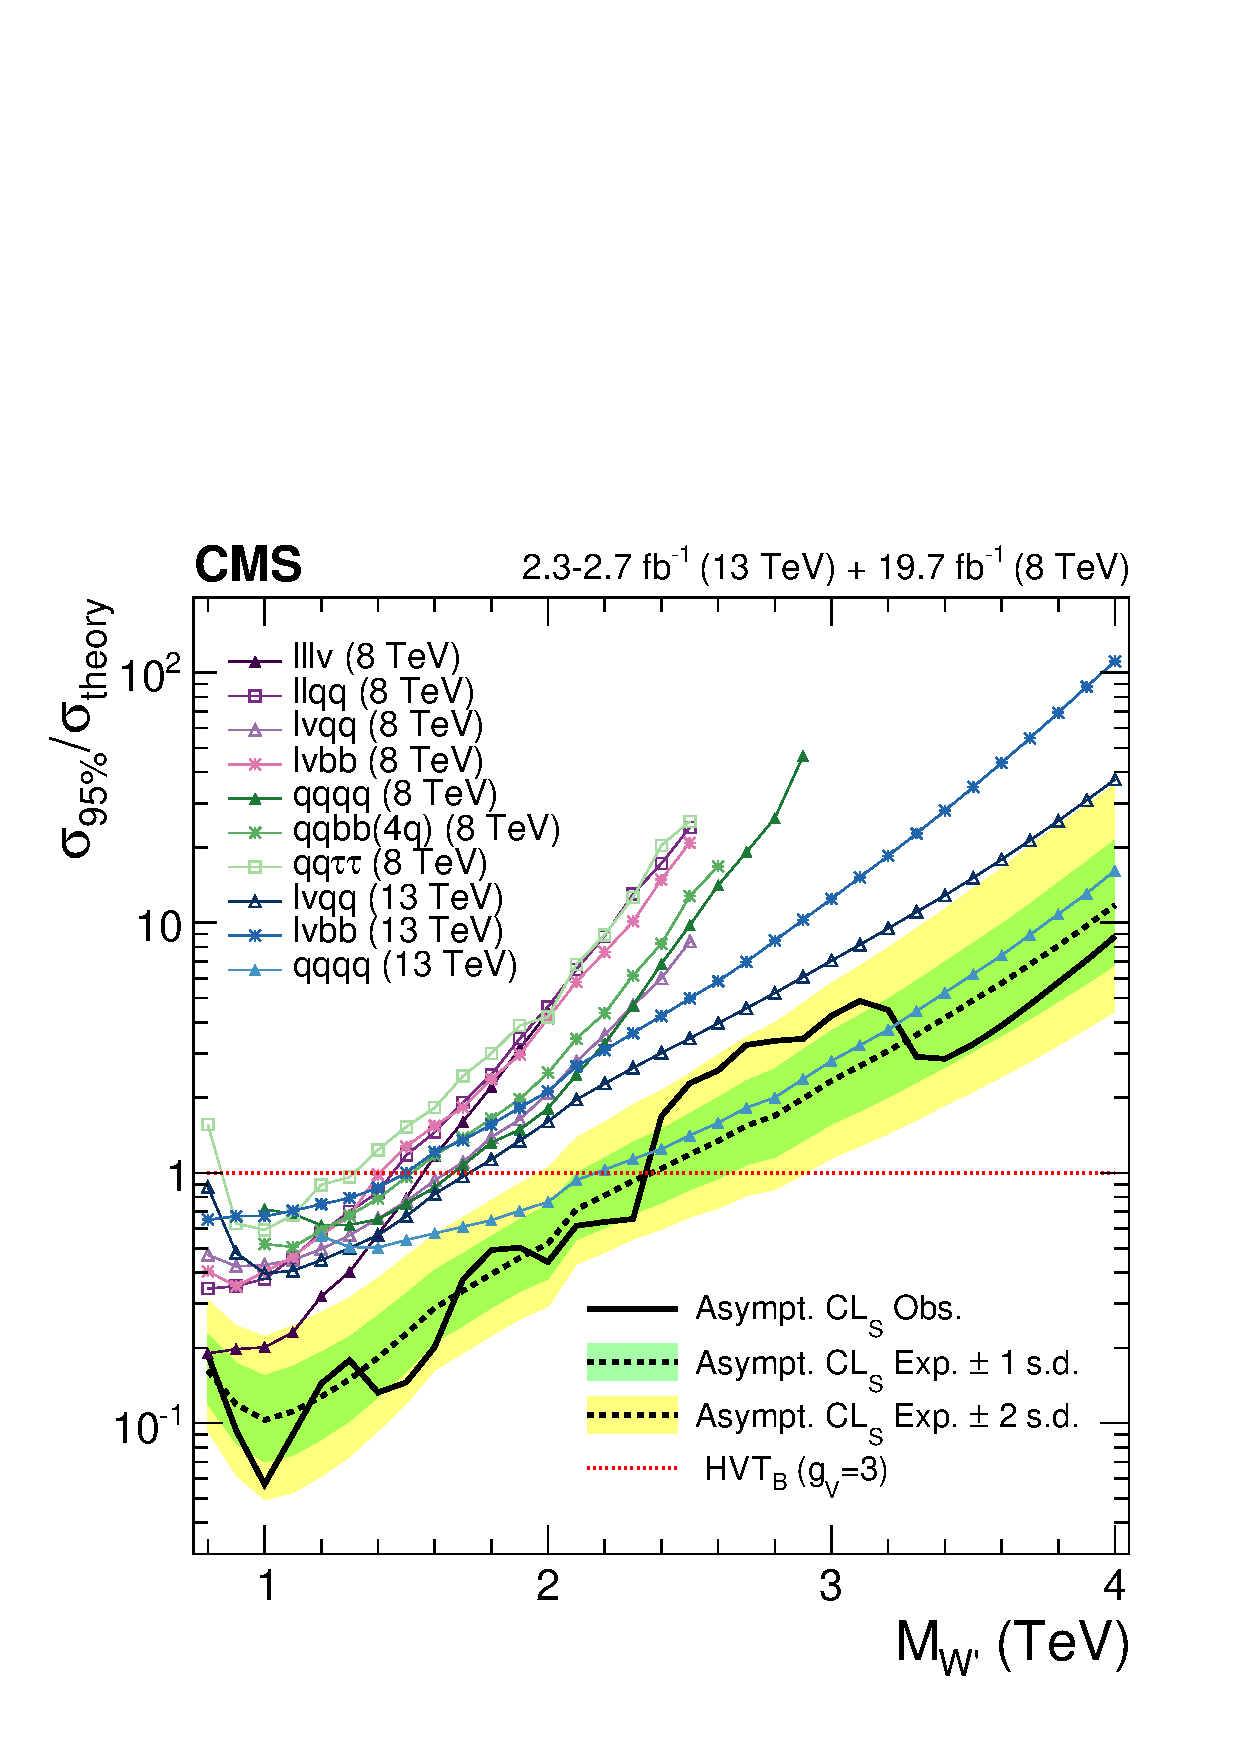
\includegraphics[width=0.45\textwidth]{\cheleven/EXOVVhvt_compare_ALLWPRIME138_final.pdf}}\\
\subfigure[]{\label{fig:wpall_138TeV_c}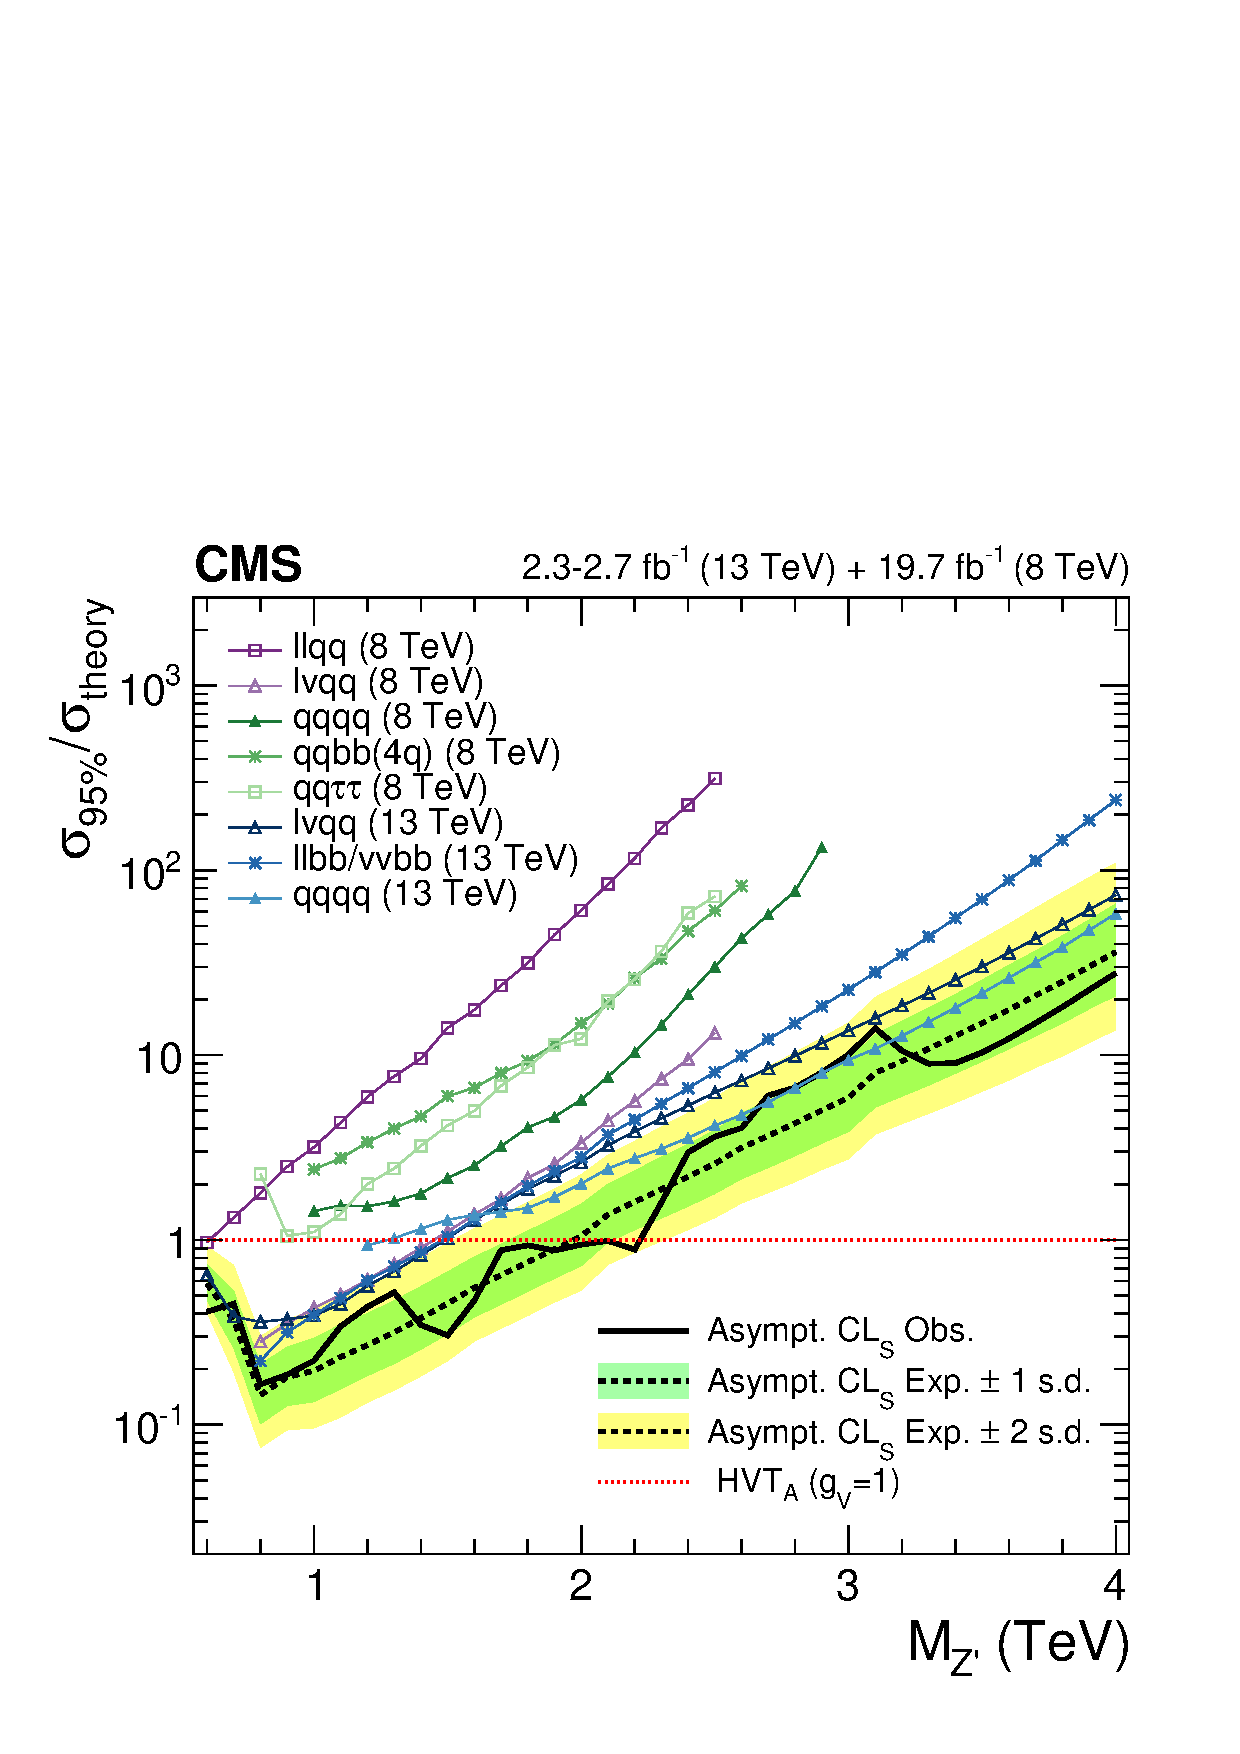
\includegraphics[width=0.45\textwidth]{\cheleven/EXOVVhvta_compare_ALLZPRIME138_final.pdf}}
\subfigure[]{\label{fig:wpall_138TeV_d}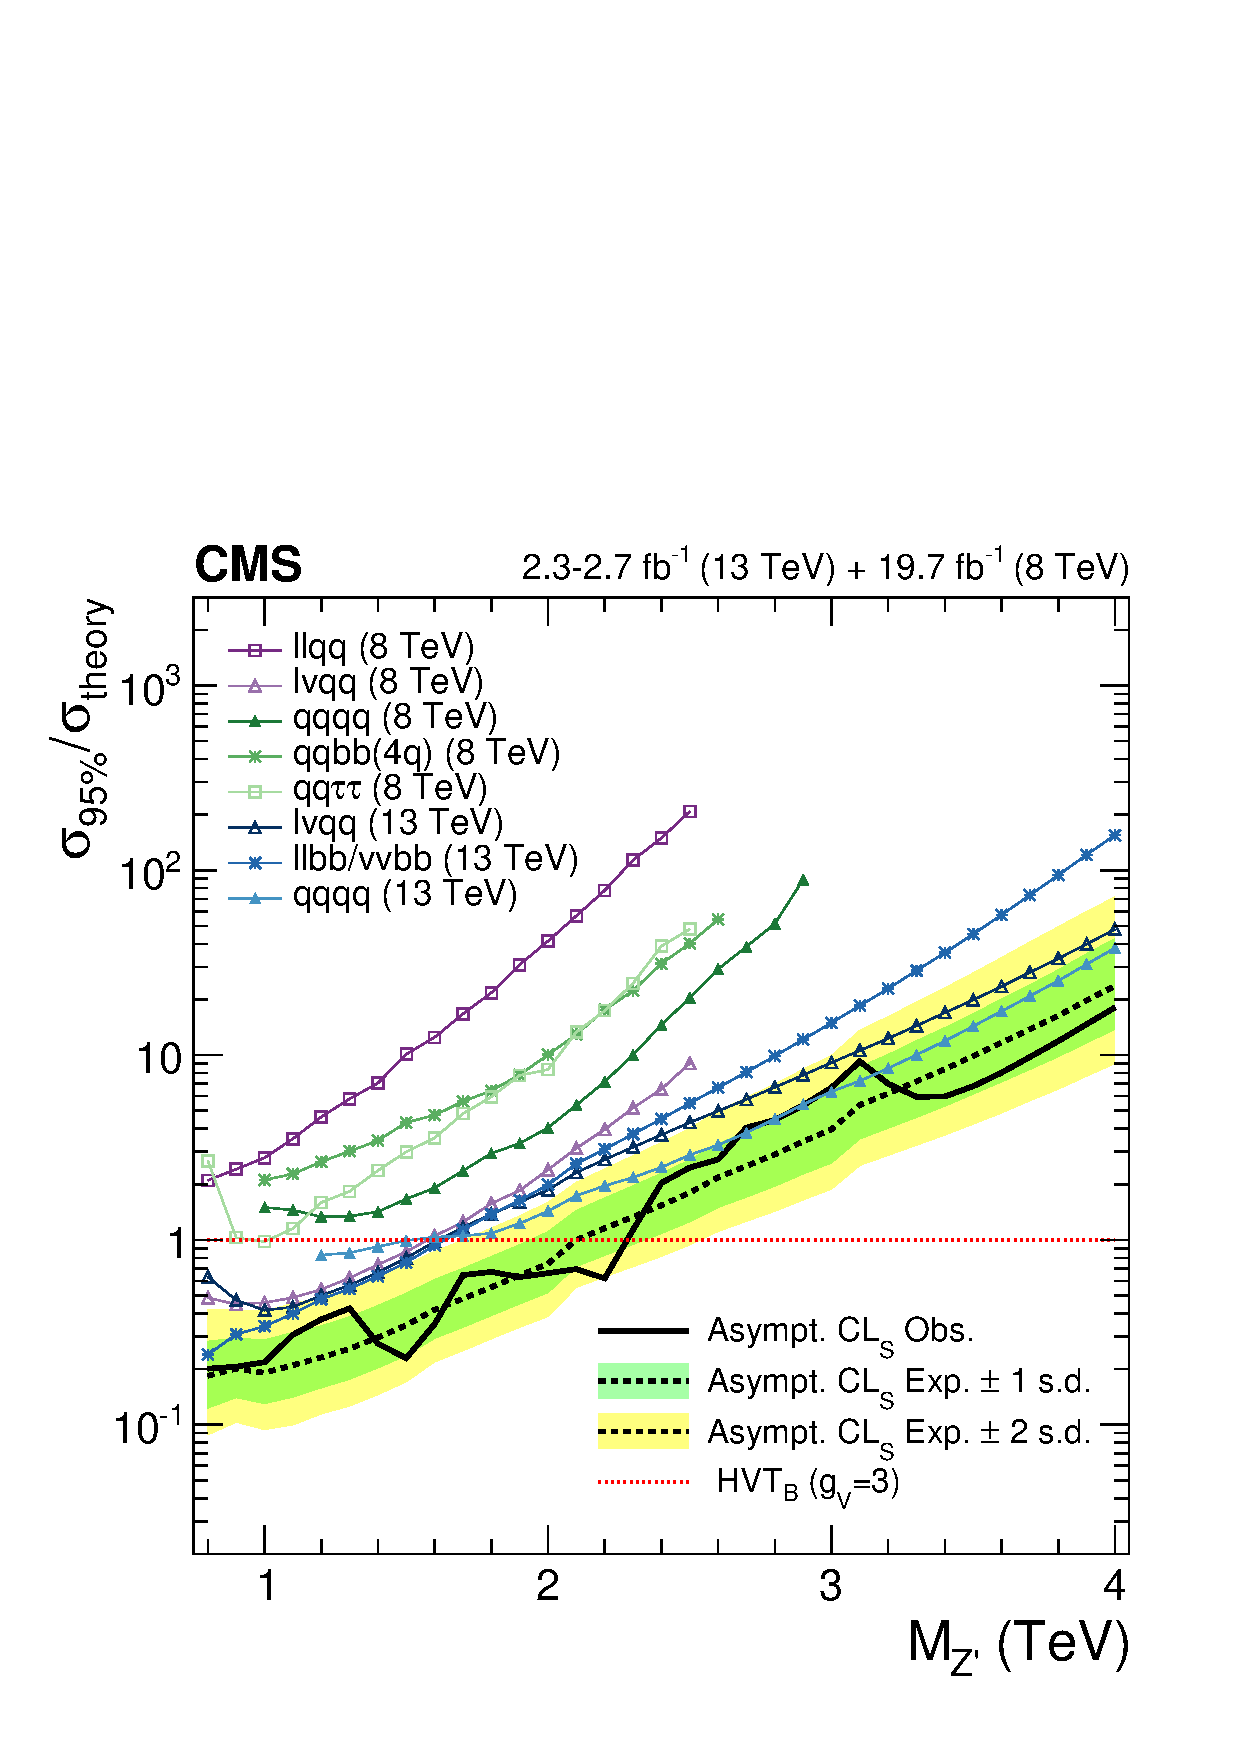
\includegraphics[width=0.45\textwidth]{\cheleven/EXOVVhvt_compare_ALLZPRIME138_final.pdf}}
\caption{%
Exclusion limits at 95\% CL on the signal strength for (top) $\Wpr \rightarrow WZ/WH$ and (bottom) $\Zpr \rightarrow WW/ZH$ in (left) HVT model A and (right) HVT model B as a function of the resonance mass obtained by combining the 8 and 13 TeV diboson searches. In each of the plots the different colored lines correspond to the searches entering the combination.}
\label{fig:wpall_138TeV}
\end{figure}

Figures~\ref{fig:wpall_138TeV_a} and~\ref{fig:wpall_138TeV_b} show the comparison and combination of the results obtained in the 8 and 13 TeV searches for a \Wpr singlet resonance for model A and model B, respectively.
The 95\% CL exclusion limits on the signal strength in the resonance mass range 0.6 $<~m_{\Wpr}~<$ 4 TeV for model A and 0.8 $<~m_{\Wpr}~<$ 4 TeV for model B are shown.
Table~\ref{tab:HVTlimits} summarizes the resulting resonance mass exclusion limits.
Below resonance mass values of about 1.4 TeV, the 3$\ell\Pgn$ channel at 8 TeV is most sensitive.
%At higher masses the $\qqbar\bbbar$ channel has approximately the same sensitivity as the $\ell \Pgn \qqbar$ and $\qqbar \qqbar$ channels.
At higher masses, the $\qqbar \qqbar$ search at 13 TeV dominates the sensitivity.
The overall sensitivity benefits from the combination up to resonance masses of about 2 TeV, lowering the cross section exclusion limit by up to a factor 1/3 when comparing to the most sensitive single channel.
Above masses of 2 TeV the 8 TeV channels do not add any significant contribution compared to the $\qqbar \qqbar$ search at 13 TeV.
%For resonance masses below 2 TeV, the sensitivity is improved by 20--70\% with respect to the 13 TeV combination and by 10--40\% compared to the 8 TeV combination.
The observed mass limit is not affected by the combination compared to that obtained from the 13 TeV searches.
However, the expected mass limit is slightly improved from 2.3 to 2.4 TeV.

\begin{table}[!htb]
  \centering
  \caption{Resonance mass 95\% CL exclusion limits in HVT model scenarios.}
  \begin{tabular}{l|c|c}
   Model & Observed limit (TeV) & Expected limit (TeV) \\    
    \hline
    \Wpr (model A)              & 2.3 & 2.1 \\
    \Zpr (model A)              & 2.2 & 2.0 \\
    HVT (\Wpr+\Zpr) (model A)    & 2.4 & 2.4 \\
    \hline
    \Wpr (model B)              & 2.3 & 2.4 \\
    \Zpr (model B)              & 2.3 & 2.1 \\
    HVT (\Wpr+\Zpr) (model B)    & 2.4 & 2.6 \\
  \end{tabular}
  \label{tab:HVTlimits}
\end{table}

Figures~\ref{fig:wpall_138TeV_c} and~\ref{fig:wpall_138TeV_d} show the comparison and combination of the results obtained in the 8 and 13 TeV searches for a \Zpr singlet resonance for model A and model B, respectively.
The $\ell \Pgn \qqbar$ channel at 8 TeV and the $\qqbar \qqbar$, $\ell \Pgn \qqbar$, $\ell\ell\bbbar$/$\Pgn\Pgn\bbbar$ channels at 13 TeV dominate the sensitivity over the whole range, with 8 and 13 TeV analyses giving almost equal contributions for masses below 2 TeV. Above this value, the sensitivity is mainly driven by the 13 TeV analyses.
Under this signal hypothesis the sensitivities reached by the 8 and 13 TeV channels are similar at low resonance masses. %Nevertheless, the combination improves the overall sensitivity by about 10--30\% for resonance masses below 2 TeV. For higher values, the sensitivity reached by the 13 TeV searches supersedes the ones reached at 8 TeV.
As for the \Wpr case, the mass limit is not affected by the combination compared to what is obtained from the 13 TeV searches.

%%%%%
\subsection{Limits on heavy vector triplet (\Wpr+\Zpr)}\label{subsec:comboHVT}
%%%%%

\begin{figure}[!htb]
\centering
\subfigure[]{\label{fig:hvtall_138TeV_a}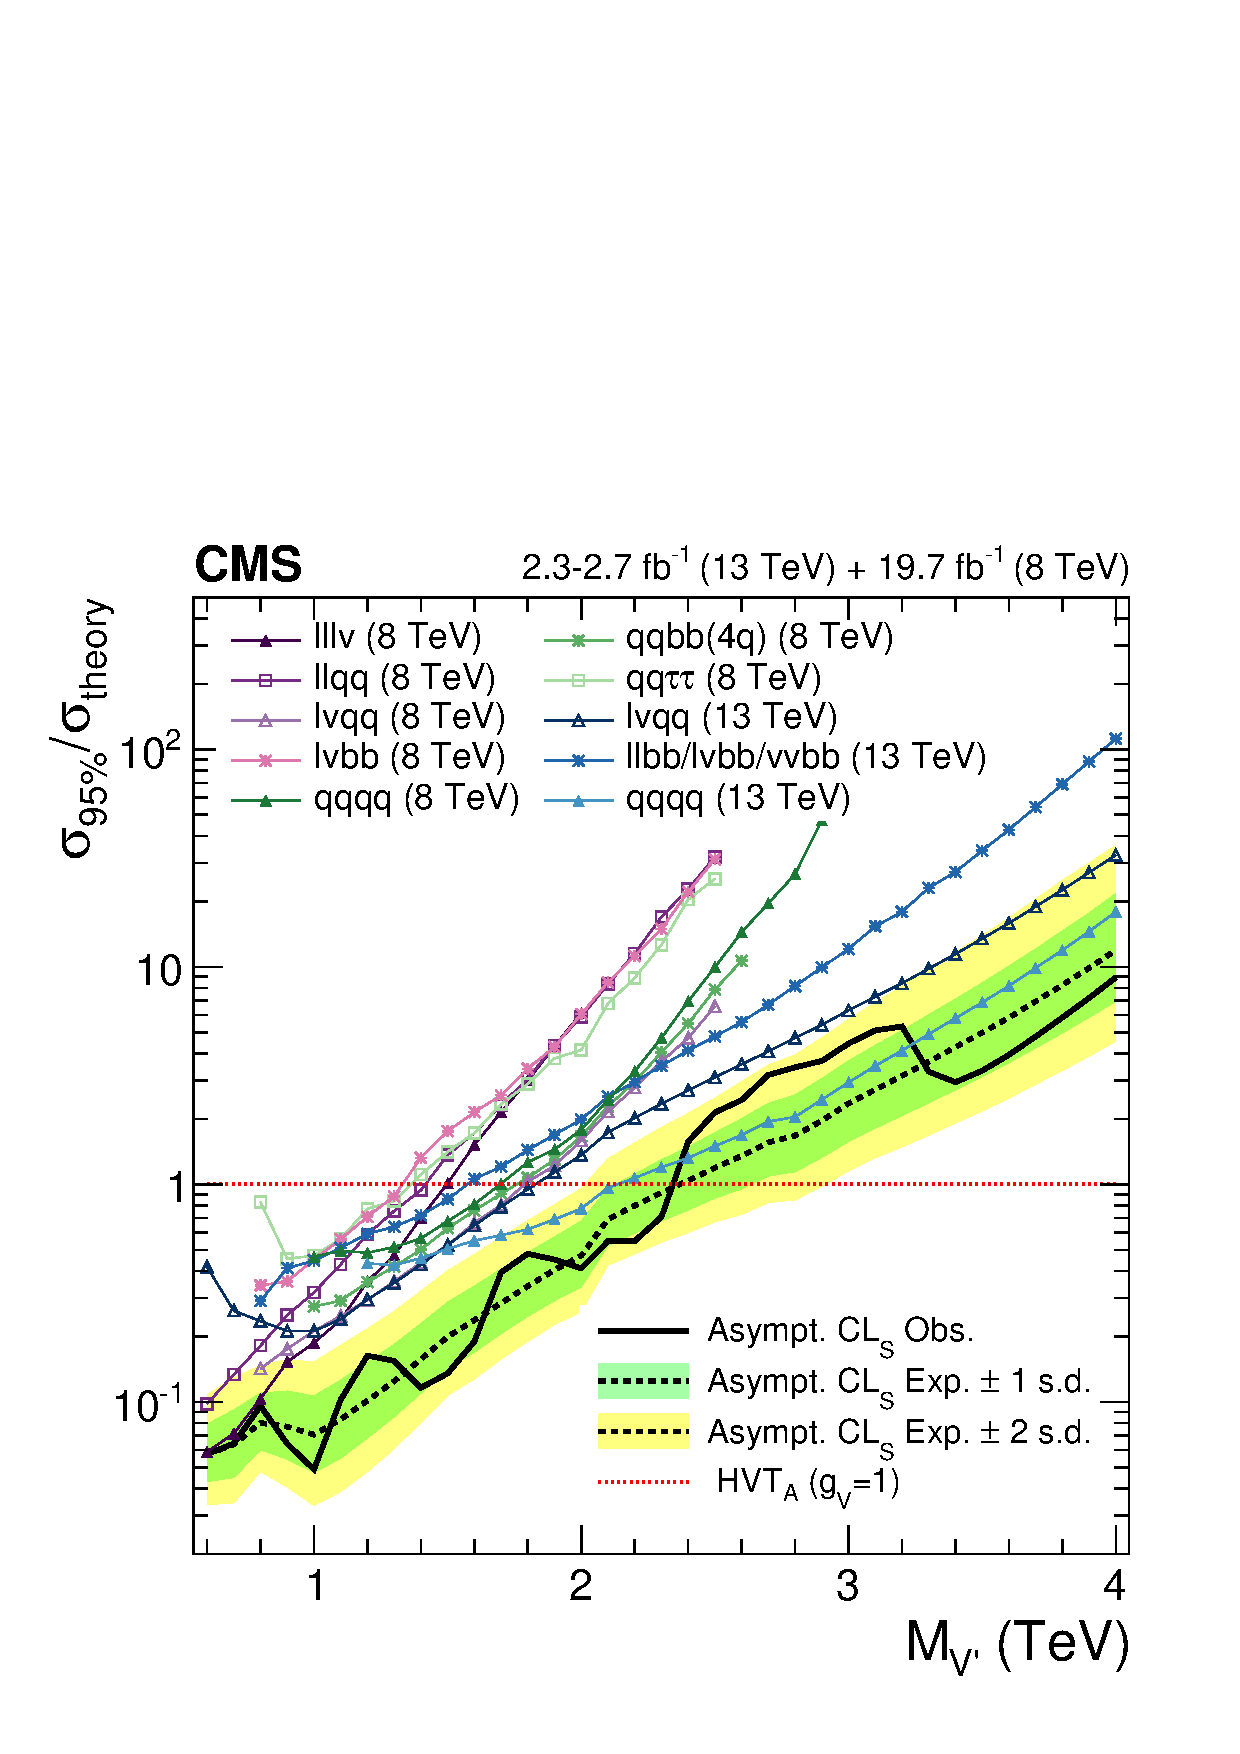
\includegraphics[width=0.45\textwidth]{\cheleven/EXOVVhvta_compare_ALLHVT138_final.pdf}}
\subfigure[]{\label{fig:hvtall_138TeV_b}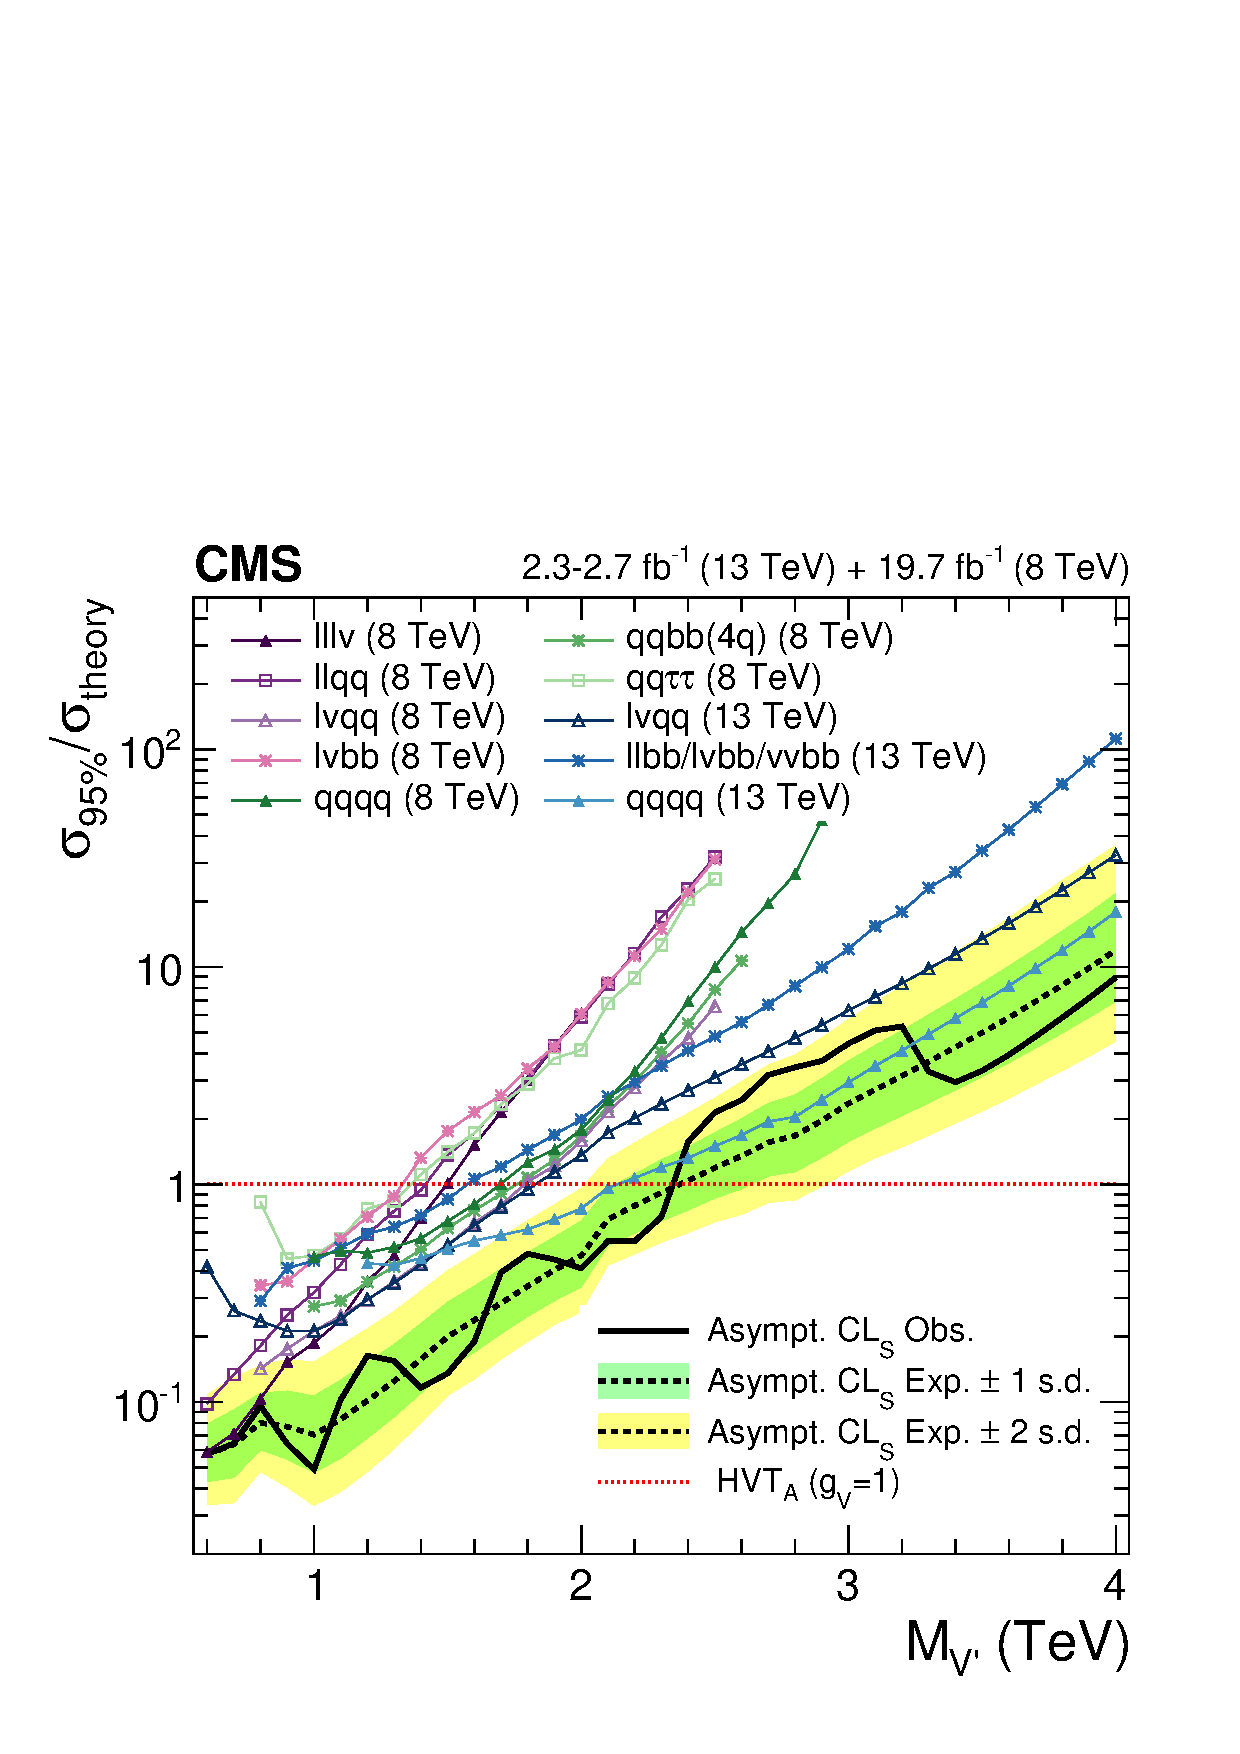
\includegraphics[width=0.45\textwidth]{\cheleven/EXOVVhvta_compare_ALLHVT138_final.pdf}}\\
\subfigure[]{\label{fig:hvtall_138TeV_c}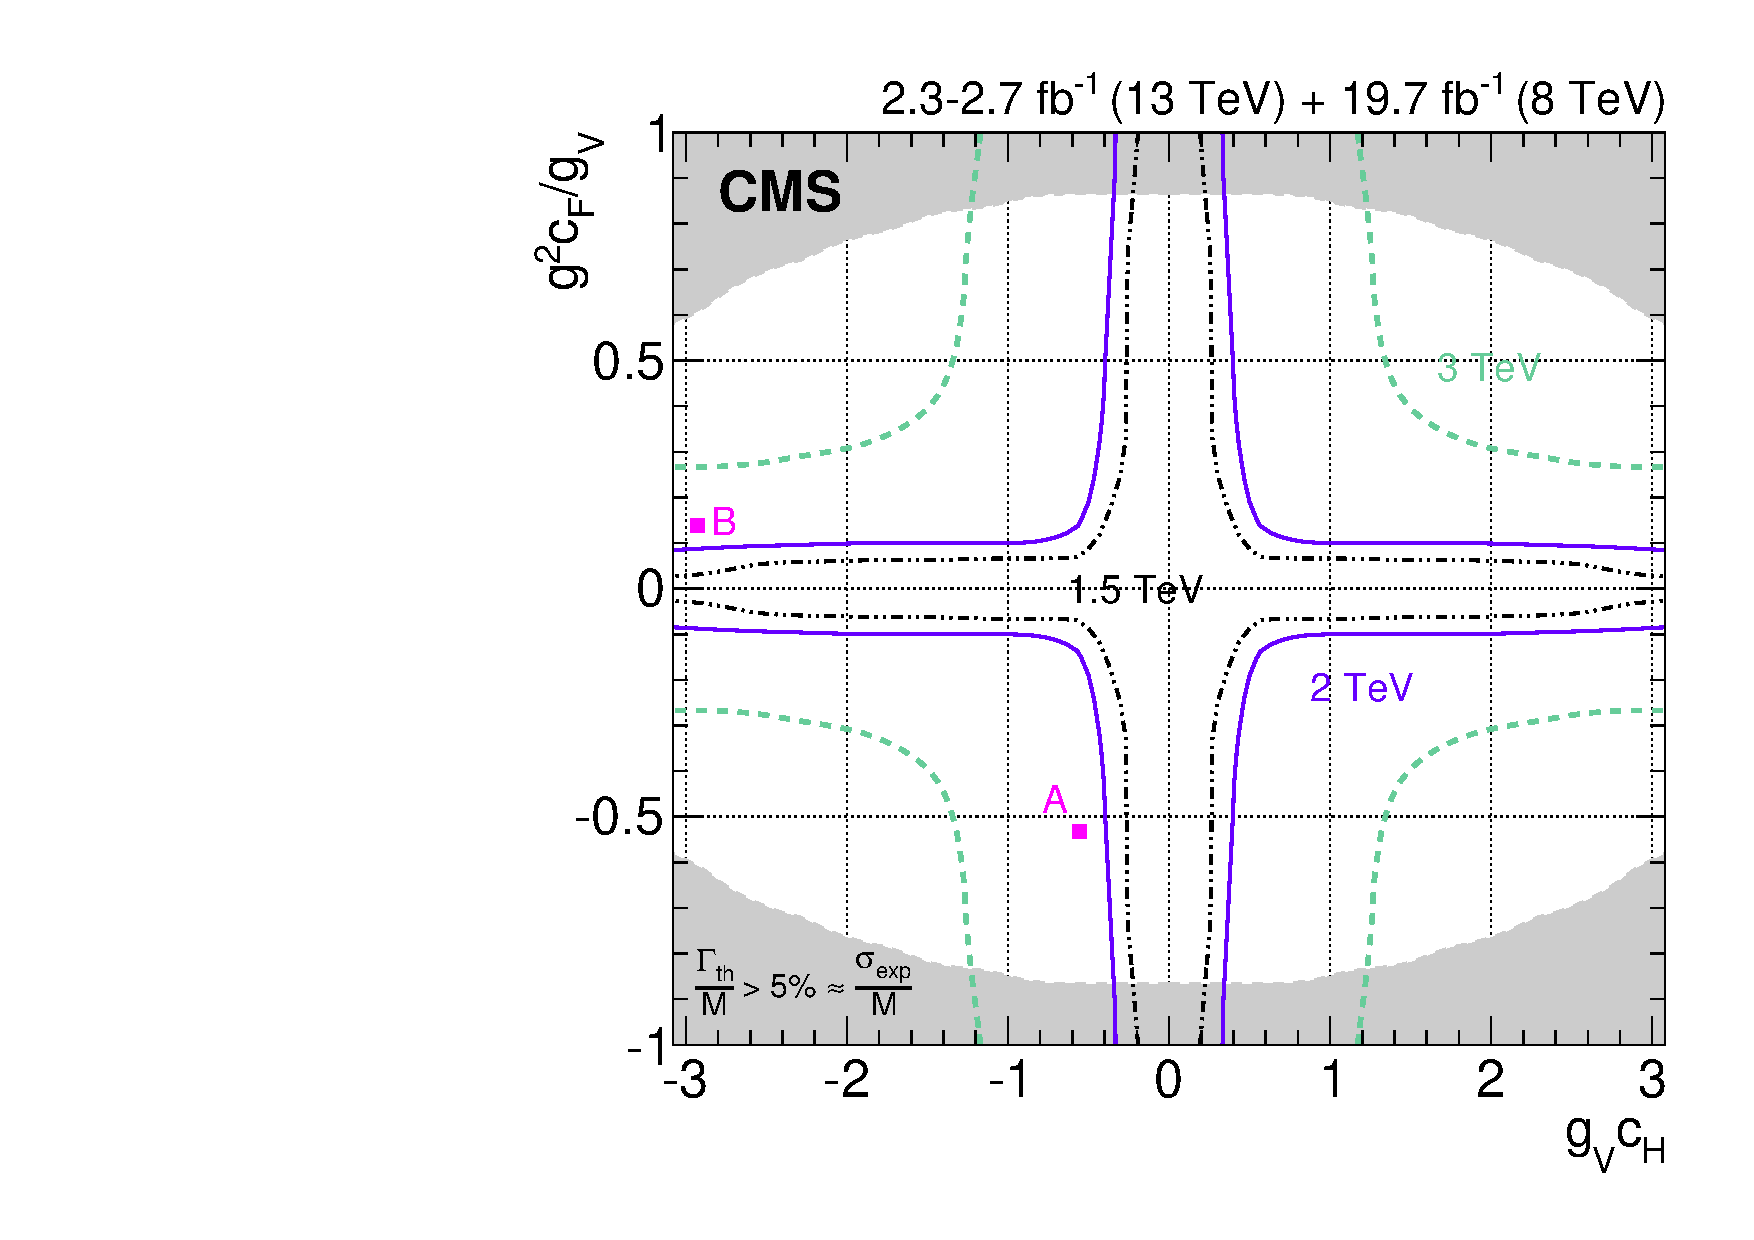
\includegraphics[width=0.45\textwidth]{\cheleven/hvt-couplings.pdf}}
\caption{
Exclusion limits at 95\% CL on the signal strength in (a) HVT model A and (b) HVT model B as a function of the resonance mass obtained by combining the 8 and 13 TeV diboson searches. In both plots the different colored lines correspond to the searches entering the combination.
(c) Exclusion regions in the plane of the HVT-model couplings ($g_{\rm V}c_{\rm H}$, $g^2c_{\rm F}/g_{\rm V}$ ) for three resonance masses, 1.5, 2, and 3 TeV, where $g$ denotes the weak gauge coupling. The points A and B of the benchmark models used in the analysis are also shown.
The boundaries of the regions outside these lines that are excluded by this search are indicated by the solid and dashed lines.
The areas indicated by the solid shading correspond to regions where the resonance width is predicted to be more than 7\% of the resonance mass and the narrow-resonance assumption is not satisfied.
}
\label{fig:hvtall_138TeV}
\end{figure}

Figures~\ref{fig:hvtall_138TeV_a} and~\ref{fig:hvtall_138TeV_b} shows the comparison and combination of the results obtained in the 8 and 13 TeV searches for a heavy vector triplet scenario.
%The $\ell \Pgn \qqbar$ channels dominate the sensitivity over the whole range together with the $\qqbar\bbbar$ channel for masses below 2 TeV.
%Above this value, the sensitivity is mainly driven by the 13 TeV analyses.
%For resonance masses below 2 TeV, the sensitivity is improved by 20--50\% with respect to the 13 TeV combination and by 10--30\% with respect to the 8 TeV combination. 
As for the \Wpr and \Zpr cases, the observed mass limit of 2.4 TeV obtained combining 8 and 13 TeV searches is determined by the 13 TeV channels.
%and it is the most stringent to date in the context of the HVT model in the B scenario.

In Fig.~\ref{fig:hvtall_138TeV_c}, a scan of the coupling parameters and the corresponding observed 95\% CL exclusion contours in the HVT model from the combination of the 8 and 13 TeV analyses are shown. The parameters are defined as $g_{\rm V}c_{\rm H}$ and $g^2c_{\rm F}/g_{\rm V}$, in terms of the coupling strengths (Section~\ref{subsec:hvt}) of the new resonance to the Higgs boson and to fermions. The range of the scan is limited by the assumption that the new resonance is narrow. A contour is overlaid, representing the region where the theoretical width is larger than the experimental resolution of the searches, and hence where the narrow-resonance assumption is not satisfied. This contour is defined by a predicted resonance width of 5\%, corresponding to the narrowest resonance mass resolution of the considered searches.

%%%%%
\subsection{Limits on bulk graviton}
%%%%%

Figure~\ref{fig:bulkgall_138TeV} shows the comparison and combination of the results obtained in the 8 and 13 TeV VV searches in the bulk graviton scenario with $k/\bar{M}_{Pl}=$~0.5.
The sensitivity is mainly driven by the 13 TeV $\qqbar \qqbar$ and $\ell \Pgn \qqbar$ channels.
%At a resonance mass of 2 TeV the sensitivity on the cross section reached by the 13 TeV searches supersedes the 8 TeV searches by factors of 2.1 and 3.6 for the $\ell \Pgn \qqbar$ and $\qqbar\qqbar$ channel, respectively. 
Under this signal hypothesis, the sensitivity reached by the 13 TeV searches supersedes the 8 TeV combination down to very low resonance masses (0.7\TeV), since this signal is produced via gluon-fusion in contrast to the HVT resonances produced via $\qqbar$ annihilation.
Hence, the contribution given by 8 TeV channels is less significant with respect to the spin-1 resonance hypotheses.
%Nevertheless, with the combination the sensitivity is improved by 10--40\% for resonance masses below 1.6 TeV.
The combination yields the most stringent signal strength limits on narrow bulk graviton resonances ($k/\bar{M}_{Pl}=$~0.5) to date in the mass range from 0.6 to 4~TeV.

\begin{figure}[!htb]
\centering
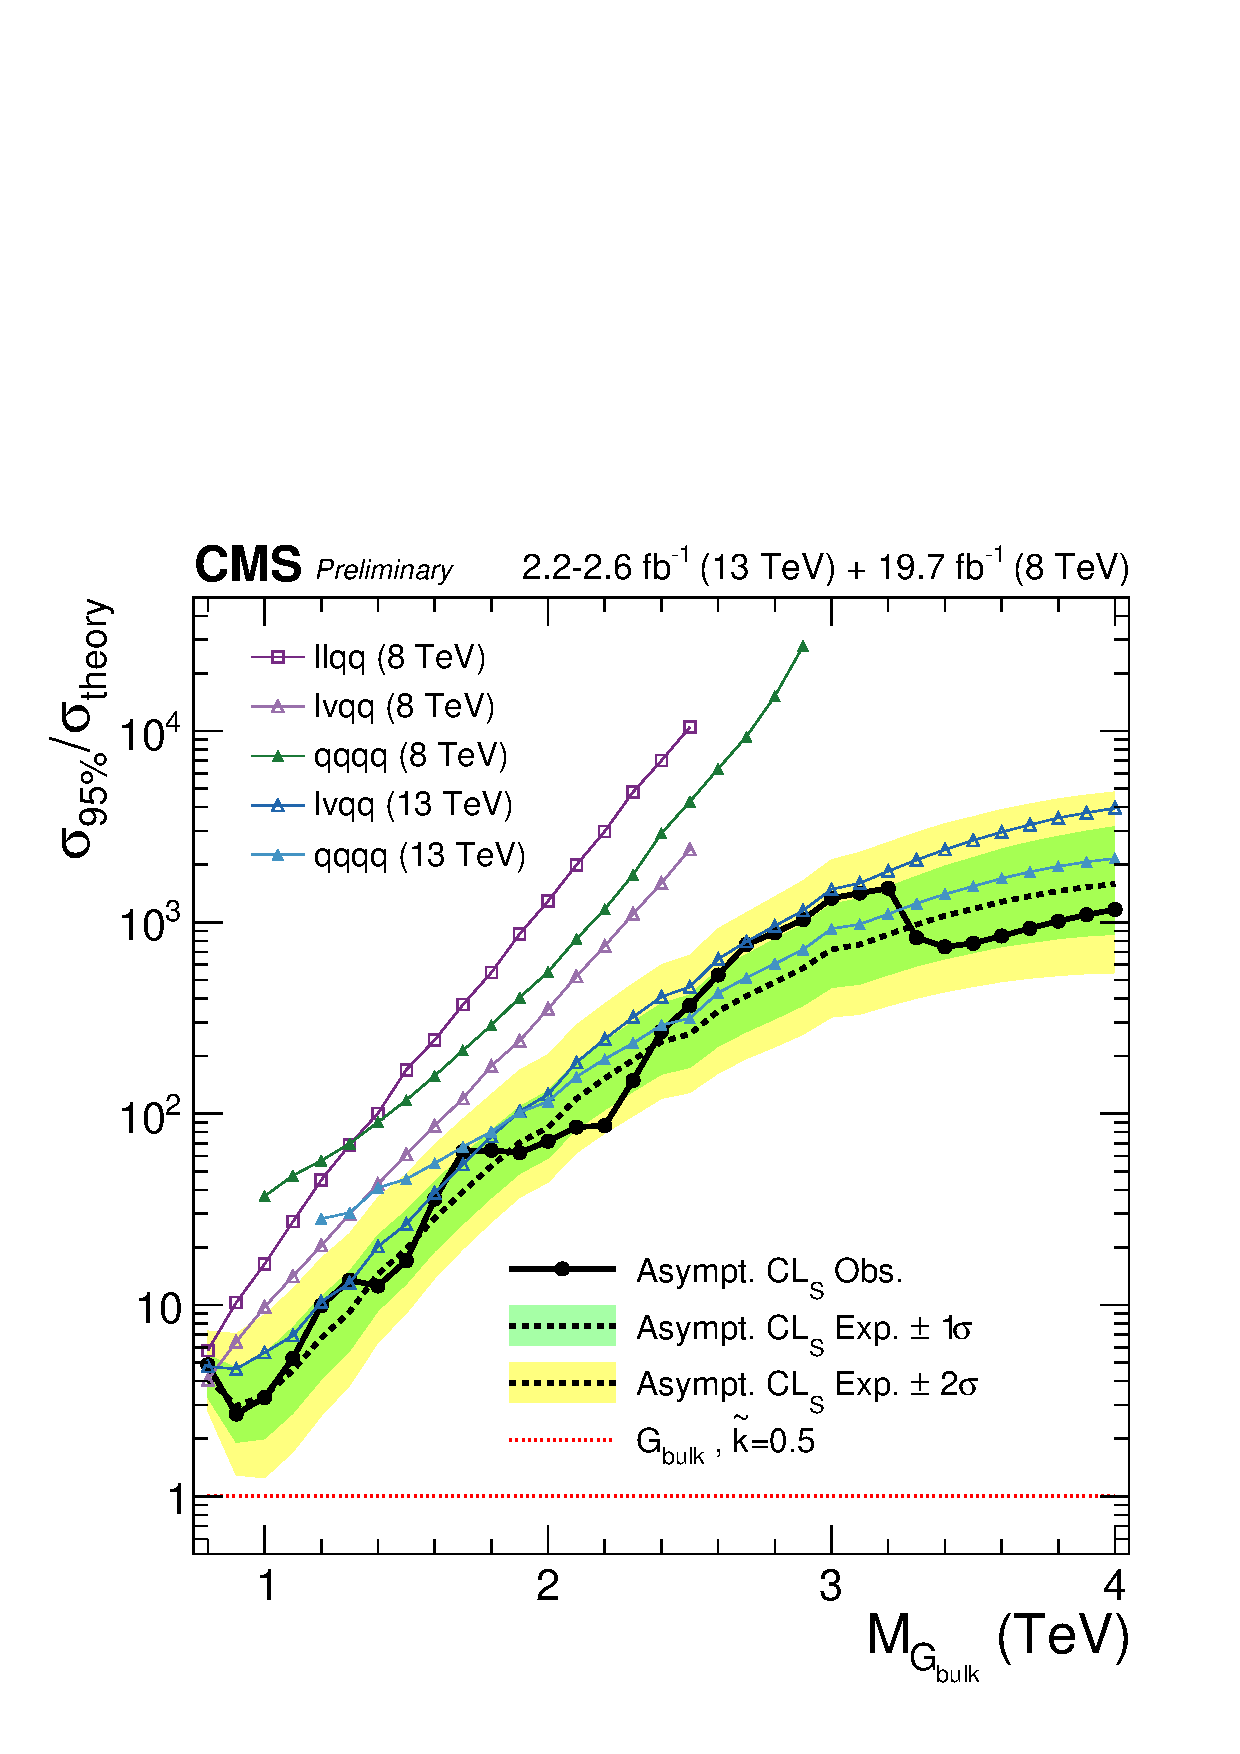
\includegraphics[width=0.45\textwidth]{\cheleven/EXOVVbulkg_compare_ALL813_final.pdf}
\caption{
Exclusion limits at 95\% CL on the signal strength as a function of the resonance mass obtained by combining the 8 and 13 TeV diboson searches in the bulk graviton scenario with $k/\bar{M}_{Pl}=$~0.5. The different colored lines correspond to the searches entering the combination.}
\label{fig:bulkgall_138TeV}
\end{figure}

%%%%%
\subsection{Significance at 2 TeV}
%%%%%

ATLAS reported an excess in the all-hadronic VV~$\to\qqbar\qqbar$ search corresponding to a local significance of 3.4$\sigma$ for a \Wpr resonance with a mass of 2 TeV~\cite{Aad:2015owa}.
For CMS, the largest deviation of 2.2$\sigma$ has been observed in the semi-leptonic WH~$\to \ell \Pgn \bbbar$ search described in this work (Chapter~\ref{ch:results8}).
The combined significance of the 8 and 13 TeV CMS searches in the range 1.8--2.0\TeV is here evaluated and showed in Figure~\ref{fig:comboSignif} for a \Wpr hypothesis.

Combining all 8 TeV VH searches in the \Wpr hypothesis, the local significance of the excess at 1.8\TeV is slightly reduced to 2.1$\sigma$.
Combining all 8 TeV VV and VH searches, it is increased back to 2.2$\sigma$, since the VV searches observed a small deviation in the same resonance mass range.
However, in combination with the 13 TeV VV and VH searches, the overall significance at 1.8\TeV is reduced to 0.8$\sigma$.
This remains the largest significance for the overall combination of 8+13 TeV searches considering all signal hypothesis over the mass range 1.8--2.0\TeV,
thus not supporting the excesses observed in the two individual channels in 8\TeV data.
%The highest overall signficance considering all signal hypotheses over the mass range 1.8--2.0\TeV is found for a \Wpr resonance at 1.8\TeV with a significance of 0.8$\sigma$.
%The combination thus does not support the excesses observed in the two individual channels in 8\TeV data.

\begin{figure}[!htb]
\centering
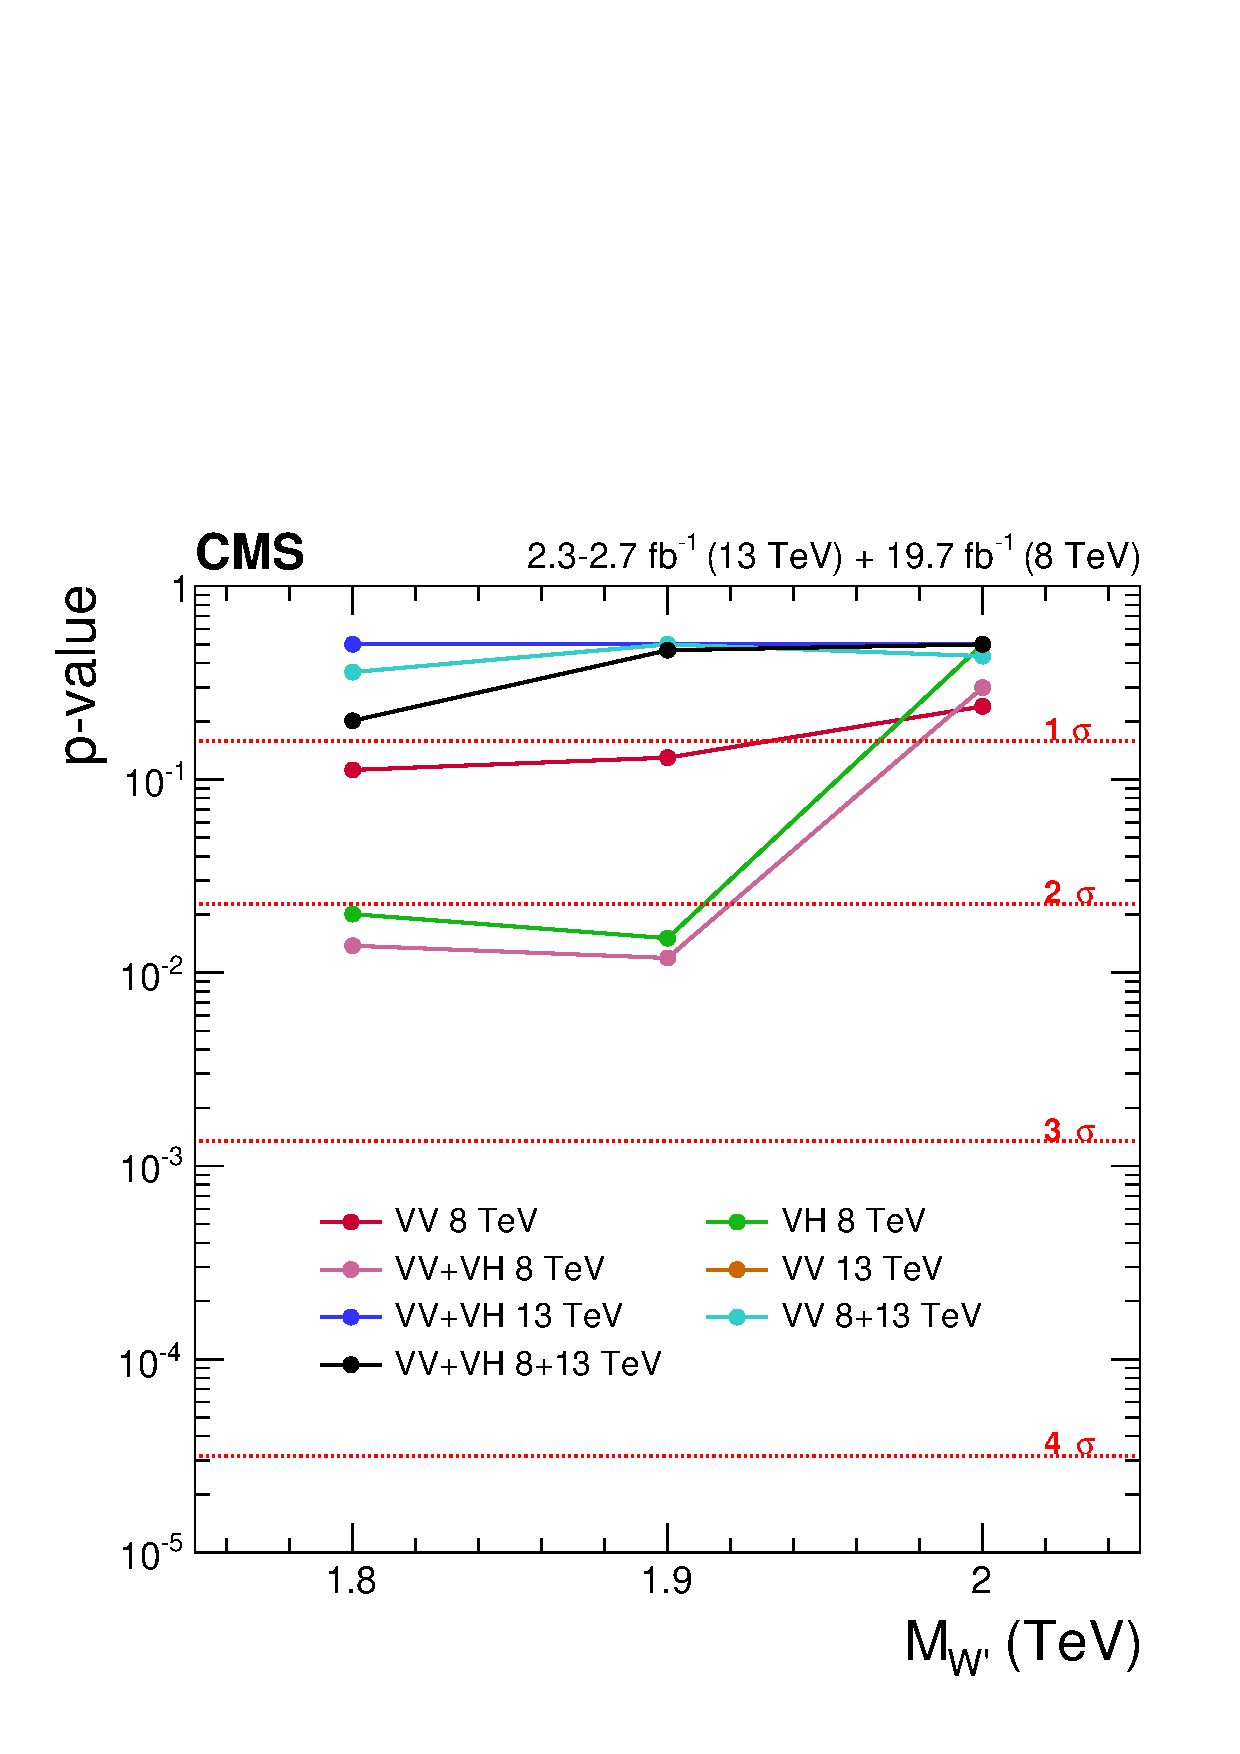
\includegraphics[width=0.45\textwidth]{\cheleven/combo-signif-wp.pdf}
\caption{Local p-values of the excesses observed in the resonance mass range 1.8--2\TeV in the various combinations of searches for a \Wpr hypothesis.}
\label{fig:comboSignif}
\end{figure}

%\begin{table}[htb]
%  \centering
%  \topcaption{Statistical significance of excesses observed at 1.8 TeV in the various combinations of searches and signal scenarios, expressed in standard deviations.}
%  \begin{tabular}{l|c|c|c|c}
%   Combination & \Wp & \Zp & HVT (\Wp+\Zp) & G$\rm_{bulk}$\\    
%    \hline
%    \hline
%    VV 8 TeV               & 1.22 & 0.64 & 1.07 & 1.61 \\
%    VH 8 TeV               & 2.05 & 0.56 & 1.79 & - \\
%    VV+VH 8 TeV            & 2.20 & 0.77 & 1.95 & - \\
%    VV 13 TeV              & 0.00 & 0.43 & 0.00 & 0.00 \\
%    VV+VH 13 TeV           & 0.00 & 0.00 & 0.00 & - \\
%    VV 8+13 TeV            & 0.36 & 0.71 & 0.54 & 0.36 \\
%    VV+VH 8+13 TeV         & 0.84 & 0.02 & 0.99 & -
%  \end{tabular}
%  \label{tab:significance_1p8TeV}
%\end{table}

%\begin{table}[htb]
%  \centering
%  \topcaption{Statistical significance of excesses observed at 1.9 TeV in the various searches, expressed in standard deviations.}
%  \begin{tabular}{l|c|c|c|c}
%   Combination & \Wp & \Zp & HVT (\Wp+\Zp) & G$\rm_{bulk}$\\     
%    \hline
%    \hline
%    VV 13 TeV             & 0.00 & 0.05 & 0.00 & 0.00 \\
%    VV+VH 13 TeV      & 0.00 & 0.00 & 0.00 & -\\
%    VV 8 TeV               & 1.20 & 0.46 & 0.91 & 1.05\\  
%    VV 8+13 TeV         & 0.00 & 0.30 & 0.00 & 0.00\\ 
%    VH 8 TeV               & 2.17 & 1.41 & 1.78 & - \\
%    VV+VH 8 TeV        & 2.32 & 1.02 & 1.89 & - \\
%    VV+VH 8+13 TeV  & 0.33 & 0.00 & 0.20 & -
%  \end{tabular}
%  \label{tab:significance_1p9TeV}
%\end{table}

%\begin{table}[htb]
%  \centering
%  \topcaption{Statistical significance of excesses observed at 2 TeV in the various searches, expressed in standard deviations.}
%  \begin{tabular}{l|c|c|c|c}
%   Combination & \Wp & \Zp & HVT (\Wp+\Zp) & G$\rm_{bulk}$\\     
%    \hline
%    \hline
%    VV 13 TeV             & 0.00 & 0.07 & 0.00 & 0.00 \\
%    VV+VH 13 TeV      & 0.00 & 0.00 & 0.00 & -\\  
%    VV 8 TeV               & 0.77 & 0.75 & 0.76 & 0.44\\
%    VV 8+13 TeV         & 0.23 & 0.45 & 0.29 & 0.06\\
%    VH 8 TeV               & 0.00 & 0.00 & 0.00 & -\\
%    VV+VH 8 TeV        & 0.58 & 0.60 & 0.48 & -\\
%    VV+VH 8+13 TeV  & 0.00 & 0.00 & 0.00 & -
%  \end{tabular}
%  \label{tab:significance_2TeV}
%\end{table}
